% !TEX root = Master.tex

Let $\mathbf{X}=\left\{X_{1}, X_{2}, \ldots, X_{p}\right\}$ be a set of \acp{RV}. A \textit{Bayesian network} is a \ac{DAG} $G = (\bm{V},A)$ where each node $v_i \in \bm{V}$ corresponds to a \ac{RV} $X_i$, $i \in \{1, \ldots, p\}$ and each arc $a = (u,v)$ corresponds to a conditional dependence between two \acp{RV}. The \textit{Markov property}, i.e. a node is conditionally independent of its non-descendants given its parents, enables the representation of the joint probability distribution of the \acp{RV} in $\bm{X}$ as a product of conditional distributions \citep{nagarajan2013bayesian}, allowing simplification of the joint distribution as a result of the \textit{chain rule} and reducing the conditional part to the parents of $X_i$. For discrete \acp{RV}, the joint probability is therefore given by 
\begin{equation}
\mathrm{P}_{\bm{\mathrm{X}}}(\mathbf{X})=
\prod_{i=1}^{p} \mathrm{P}_{X_i}\left(X_{i} \mid X_{1}, \ldots, X_{i-1}\right) =
\prod_{i=1}^{p} \mathrm{P}_{X_{i}}\left(X_{i} \mid \Pi_{X_{i}}\right),
\end{equation}
where $\Pi_{X_{i}}$ is the set of the parents of $X_i$. For continuous \acp{RV}, we can write the joint density of $f_{\mathbf{X}}$ as
\begin{equation}
f_{\mathbf{X}}(\mathbf{X})=
\prod_{i=1}^{p} f_{X_i}\left(X_{i} \mid X_{1}, \ldots, X_{i-1}\right) =
\prod_{i=1}^{p} f_{X_{i}}\left(X_{i} \mid \Pi_{X_{i}}\right).
\end{equation}
\\

In real-world settings, entities often represent variables which vary over time. \textit{\acp{DBN}} extend the framework of static Bayesian networks to model associations arising from temporal dynamics between such entities \citep{nagarajan2013bayesian}. Each \ac{RV} in a \ac{DBN} is represented by several nodes across time-points. In the \ac{DAG} resulting from a \ac{DBN}, arcs can be drawn between variables across successive time-points (or at the same time-point,\footnote{In \cite{nagarajan2013bayesian}) conditional dependencies can occur only between successive time-points. However, this assumption is relaxed here due to practical alignments coming up in Section \ref{ssec:article_dependencies}.} as long as no arc is enters an ancestor node). The arcs in the \ac{DAG} describe exactly the conditional dependencies between any pair of variables given the past variables (or variables at the same time stage). \autoref{fig:dynamic_bn} represents a graphical example of such a \ac{DBN}.
\\


\begin{figure}[H]
\centering
  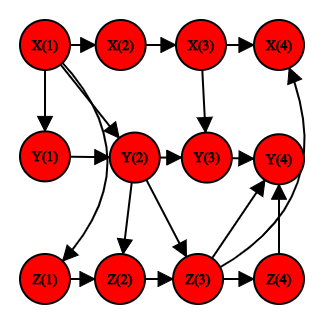
\includegraphics[width=0.45\linewidth]{figures/dynamic_bn.png}
  \caption{Graphical representation of a time-varying dynamic Bayesian network of three random variables ($X$, $Y$ and $Z$) with four time periods}
  \label{fig:dynamic_bn}
\end{figure}


Dependence relationships in \acp{DBN} are often represented by a \ac{VAR} process as in \autoref{eq:multivariate_ts}. Assuming a \ac{VAR}(1) process with $k$ variables, each variable $X_i$, $i = 1,\ldots,k$ satisfies
\begin{equation}
X_{i}(t)=\sum_{j=1}^{k} a_{i j} X_{j}(t-1)+b_{i}+\varepsilon_{i}(t) \quad \text { where } \quad \varepsilon_{i}(t) \sim N\left(0, \sigma_{i}(t)\right),
\end{equation}
where all arcs are defined between two consecutive time-points. The set of non-zero coefficients $a_{ij}$ in an auto-regressive matrix $A$ define the arc set, meaning that if element $a_{ij}$ is non-zero, the network includes an arc from $X_i$ to $X_j$. Repeated measurements can be used to perform linear regression, however the ordinary least square estimates of the regression coefficients $a_{ij}$ and $b_i$ can be computed only when the number of time-points $n \gg k$.





